%% start of file `template.tex'.
%% Copyright 2006-2013 Xavier Danaux (xdanaux@gmail.com).
%
% This work may be distributed and/or modified under the
% conditions of the LaTeX Project Public License version 1.3c,
% available at http://www.latex-project.org/lppl/.

\documentclass[11pt,a4paper,sans]{moderncv}        % possible options include font size ('10pt', '11pt' and '12pt'), paper size ('a4paper', 'letterpaper', 'a5paper', 'legalpaper', 'executivepaper' and 'landscape') and font family ('sans' and 'roman')

% moderncv themes
\moderncvstyle{classic}                             % style options are 'casual' (default), 'classic', 'oldstyle' and 'banking'
\moderncvcolor{orange}                               % color options 'blue' (default), 'orange', 'green', 'red', 'purple', 'grey' and 'black'
%\renewcommand{\familydefault}{\sfdefault}         % to set the default font; use '\sfdefault' for the default sans serif font, '\rmdefault' for the default roman one, or any tex font name
\usepackage{xcolor,soul,wrapfig}


% character encoding
\usepackage[utf8]{inputenc}                       % if you are not using xelatex ou lualatex, replace by the encoding you are using

% adjust the page margins
\usepackage[scale=0.89]{geometry}

% personal data
\name{Thomas}{Campistron}
\address{3 rue Claude Debussy}{59800 Lille}{France}
\phone[mobile]{+33~(0)6 99 73 07 40}                % optional, remove / comment the line if not wanted
\email{irevoire@protonmail.ch}                      % optional, remove / comment the line if not wanted
\homepage{irevoire.ovh}                      % optional, remove / comment the line if not wanted
\social[github]{irevoire}                 % optional, remove / comment the line if not wanted

\newcommand{\mhref}[2]{\href{#1}{\ul{#2}}}


%----------------------------------------------------------------------------------
%            content
%----------------------------------------------------------------------------------
\begin{document}
%-----       resume       ---------------------------------------------------------
\fontdimen2\font=0.5ex% inter word space
\fontdimen3\font=0.5ex% inter word stretch

\makecvtitle

\vspace*{-0.1cm}
\section{Education}
	\cventry{
		2014--2019\\
		\vspace*{0.2cm}
		\hspace*{-0.5cm}
		\href{https://univ-lille.fr/}{
\includegraphics[width=1.0cm]{univ}}
	}{MSc in Computer Science}{\mhref{https://www.univ-lille.fr/}{University of Lille}}{France}{}{
		\textit{Relevant coursework:} Virtualization, cloud computing, distributed systems, OS design, system programming, computer architecture, compilation, cryptography
		}

\section{Work Experience}
	\cventry{
		\hspace*{-0.5cm}
		Mar 2021 -- Now\\
		\vspace*{1.5cm}
		\hspace*{-0.7cm}
		\href{https://www.meilisearch.com/}{
\includegraphics[width=2.0cm]{meilisearch}}
	}{Core team developer}{\mhref{https://www.meilisearch.com/}{Meilisearch}}{Remote}{}{
			\mhref{https://github.com/meilisearch/meilisearch}{Meilisearch is an open-source}
			search engine written in rust. I work as much on \mhref{https://github.com/meilisearch/meilisearch}{meilisearch}
			as on \mhref{https://github.com/meilisearch/milli}{milli} (the core library of meilisearch).
			I wrote all the benchmarks, set up a CI to execute the benchmarks on each commit, and push the result to see all
			the unexpected performance changes. I also fuzzed multiple parts of Meilisearch or milli to reproduce contributors' bugs without any dataset.
			Here is a little list of fun things I did;
			I implemented the indexing and searching part of the \mhref{https://docs.meilisearch.com/learn/advanced/geosearch.html\#preparing-documents-for-location-based-search}{geosearch},
			I rewrote the parser entirely for our \mhref{https://docs.meilisearch.com/learn/advanced/filtering_and_faceted_search.html\#using-filters}{filters} and drastically improved the error messages;
			We found two tricky bugs and one memory leak in our utilization of \mhref{http://www.lmdb.tech/doc/}{LMDB}
			where I used \mhref{https://rr-project.org}{RR} to understand what was going wrong with this \mhref{https://github.com/LMDB/lmdb/blob/mdb.master/libraries/liblmdb/mdb.c\#L7558-L8083}{endless, hideous and goto polluted C code}.
			\\
			On a day-to-day basis, I work with contributors, I answer questions on github issues, discussions or our community slack channel.
			I fix bugs, refactorize the code, create tooling, improve the CI and do everything you would expect from a developer.
			Sometimes I read scientific articles and publications on new DBs or distributed systems.
	}

	\cventry{
		\hspace*{-0.5cm}
		Mar--Aug 2020\\
		\href{https://www.huawei.com/}{
\includegraphics[width=1.7cm]{huawei}}
		}{Improve the performance of \mhref{https://e.huawei.com/en/products/cloud-computing-dc/atlas/mindspore}{Mindspore}}{\mhref{https://www.huawei.com}{Huawei}}{Remote}{}{
			\mhref{https://gitee.com/mindspore/mindspore}{MindSpore is an open-source}
			AI computing framework that implements a lot of state-of-the-art technologies.
			I was hired to work on an OCaml PoC for simplifying mathematical operations
			on the control flow graph of MindSpore. The aim of the project is also to
			maximize the parallelization of the programs and hence get the maximum perfs out of the
			\mhref{https://www.huawei.com/en/news/2019/8/huawei-ascend-910-most-powerful-ai-processor}{Huawei Ascend processor}
			or any gpu.
	}

	\cventry{
		\hspace*{-0.5cm}
		Mar--Aug 2019\\
		\vspace*{0.1cm}
		% \hspace*{-0.8cm}
		\href{https://worldline.com/}{
\includegraphics[width=1.7cm]{worldline}}
		}{Evaluation of the P4 Language for DDoS mitigation}{\mhref{https://worldline.com/}{Worldline}}{Lille}{}{
			Worldline is one of the European leaders of digital payments.
			The first aim of this internship was to test a new language called P4.
			This language stands for “Programming Protocol-Independent Packet Processors”.
			Our test case was to implement a SynCookie Proxy and to test it against handmade XDP or DPDK solutions.
	}

	\cventry{
		\hspace*{-0.5cm}
		Apr--Aug 2017\\
		\vspace*{0.2cm}
		\href{https://www.stormshield.com/}{
\includegraphics[width=1.2cm]{stormshield}}
		}{Optimizing and storing the Firewall rules}{\mhref{https://www.stormshield.com/}{StormShield}}{Lille}{}{
			Stormshield is a European leader in digital infrastructure security, they sell hardware Firewalls.
			My internship was about optimizing the access to the Firewall rules.
			Rules are now accessible in read-only by multiple daemons at the same time without any mutex,
			memory or loading time in $O(log_{2}(n))$ instead of $O(n^{2})$.
}


\section{Technologies}
	\cvitemwithcomment{\textbf{C}}{< 100 000 LoC}{
		My professional experience at StormShield was almost entirely in C.
		I also used C for some personal projects and during my education. I worked with OpenMPI, Valgrind, gdb, SDL2, AFL.
		I did a bit of IoT with it and it was my main go-to language until I discovered Rust.
	}
	\cvitemwithcomment{Ruby, Python}{< 10 000 LoC}{
		Mostly used as scripting languages.
		I know how to extend ruby with C and I did a little bit of C ffi in python.
		I developed a \mhref{https://github.com/sophie-kaleba/turbo-air-dryer}{JIT compiler for a subset of a language in ruby}.
	}
	\cvitemwithcomment{Haskell, VHDL, Prolog}{< 2000 LoC}{I enjoyed these languages a long time ago but do not work with it. I would love to though.}
	\cvitemwithcomment{OCaml}{< 10 000 LoC}{
		I learned the OCaml language specifically for my last job at Huawei and apart from some little personal
		project I used it almost exclusively for this project.
	}
	\cvitemwithcomment{\textbf{Rust}}{< 150 000 LoC}{
		That’s the only language I used for the last 3 years and I plan to continue working with it for a few more years.
		Here is some old project I did with friends or alone;
		\mhref{https://github.com/irevoire/teensy}{A bare-metal Rust crate}
		to easily program a \mhref{https://www.pjrc.com/store/teensy32.html}{teensy3.2}.
		We’ve also worked on a working async \mhref{https://github.com/irevoire/mindelbrust}{subset of a Minecraft server.}
		I also developed the \mhref{https://github.com/irevoire/mandelbrust}{Mandelbrot} and \mhref{https://github.com/irevoire/rulia}{Julia set} using parallelization and SIMD.
		I developed a \mhref{https://github.com/irevoire/chrustip-8}{chip-8}, \mhref{https://github.com/irevoire/esolangs}{brainfuck, Argh! interpreters}.
		I also often participate in some problem-solving challenges like \mhref{https://github.com/irevoire/project_euler}{project Euler} and \mhref{https://github.com/irevoire/aoc}{advent of code}
		or the Google Hashcode.
	}

\pagebreak
\section{Personal}
	\cvitem{\hskip -0.5cm On my free time}{
		I enjoy thinking of high performance and parallelized code, profiling code to find bottlenecks and then
		trying to apply as many techniques as possible going from optimizing the algorithm/data
		structure to things like data-oriented programming, branchless programming, multi-thread or SIMD.
		I also like bare-metal embedded system (even if I’m not that good at reading the constructor specs).
		Language and networking are also two domains that draw my attention a lot.
	}
	\cvitem{Travel}{
		I love to travel, so far I visited the following countries:
		\begin{itemize}
			\item USA -- Chicago: 2 months
			\item Japan -- Tokyo-Kyoto: 1 month
			\item Ireland -- Dublin: 2 weeks
			\item Norway -- Bergen: 1 week
			\item Finally, I went back to Japan for 2 more months
				(September–November 2019) right after my graduation
				and visited a lot of cities!
		\end{itemize}
		But also when it's possible I love to go hiking in the south of
		France or do bike trips around my city, my longest trip was ~160Km
		in one day but I usually stay below 100Km per day.
	}
	\cvitem{Other}{
		I listen to \textbf{a lot} of music. I'm almost always listening to something, usually from the 70'.
		\linebreak
		I also love good food, and especially good cheeses, cooking or playing video games.
		And finally, I have a strange addiction for keyboards that runs on
		\mhref{https://github.com/qmk/qmk_firmware/}{QMK}, currently, I own
		an \mhref{https://ergodox-ez.com/}{ergodox-ez}, a
		\mhref{https://olkb.com/products/preonic-pcb}{preonic} and I should
		get a \mhref{https://splitkb.com/collections/featured-products/products/kyria-acrylic-plate-case}{Kyria}
		in the following days.
	}
	\vskip 1cm
	\center{Here is my preonic}
	\vskip 0.5cm
	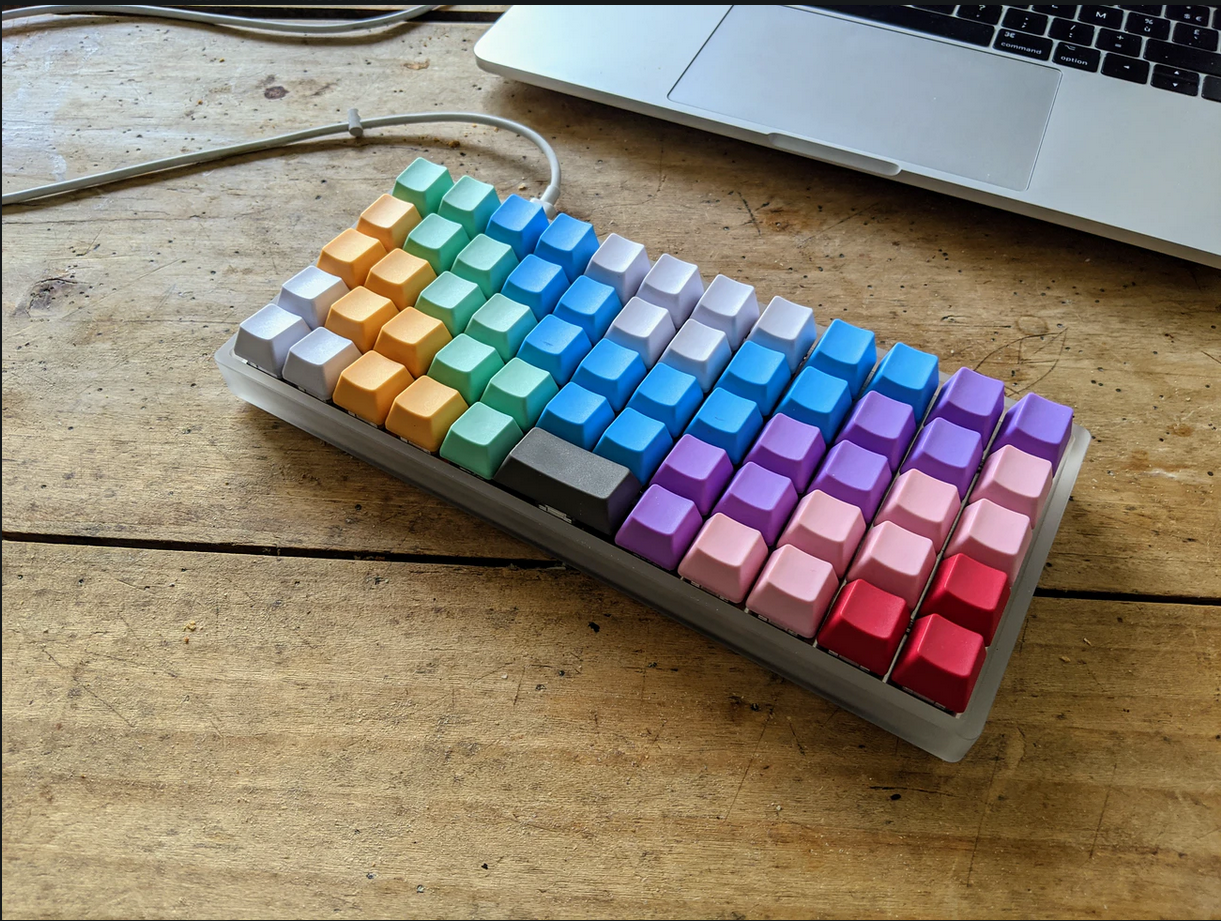
\includegraphics[width=\textwidth]{preonic}

% Publications from a BibTeX file without multibib
%  for numerical labels: \renewcommand{\bibliographyitemlabel}{\@biblabel{\arabic{enumiv}}}% CONSIDER MERGING WITH PREAMBLE PART
%  to redefine the heading string ("Publications"): \renewcommand{\refname}{Articles}
\nocite{*}
\bibliographystyle{plain}
\bibliography{publications}                        % 'publications' is the name of a BibTeX file

% Publications from a BibTeX file using the multibib package
%\section{Publications}
%\nocitebook{book1,book2}
%\bibliographystylebook{plain}
%\bibliographybook{publications}                   % 'publications' is the name of a BibTeX file
%\nocitemisc{misc1,misc2,misc3}
%\bibliographystylemisc{plain}
%\bibliographymisc{publications}                   % 'publications' is the name of a BibTeX file

\clearpage

\end{document}


%% end of file `template.tex'.
